\section{实验环境建立}
\subsection{Linux下CodeBlocks反汇编(10分)}
CodeBlocks运行hellolinux.c。反汇编查看printf函数的实现。
要求:C、ASM、内存(显示hello等内容)、堆栈(call printf前)、寄存器同时在一个窗口。

\begin{figure}[H]
	\centering
	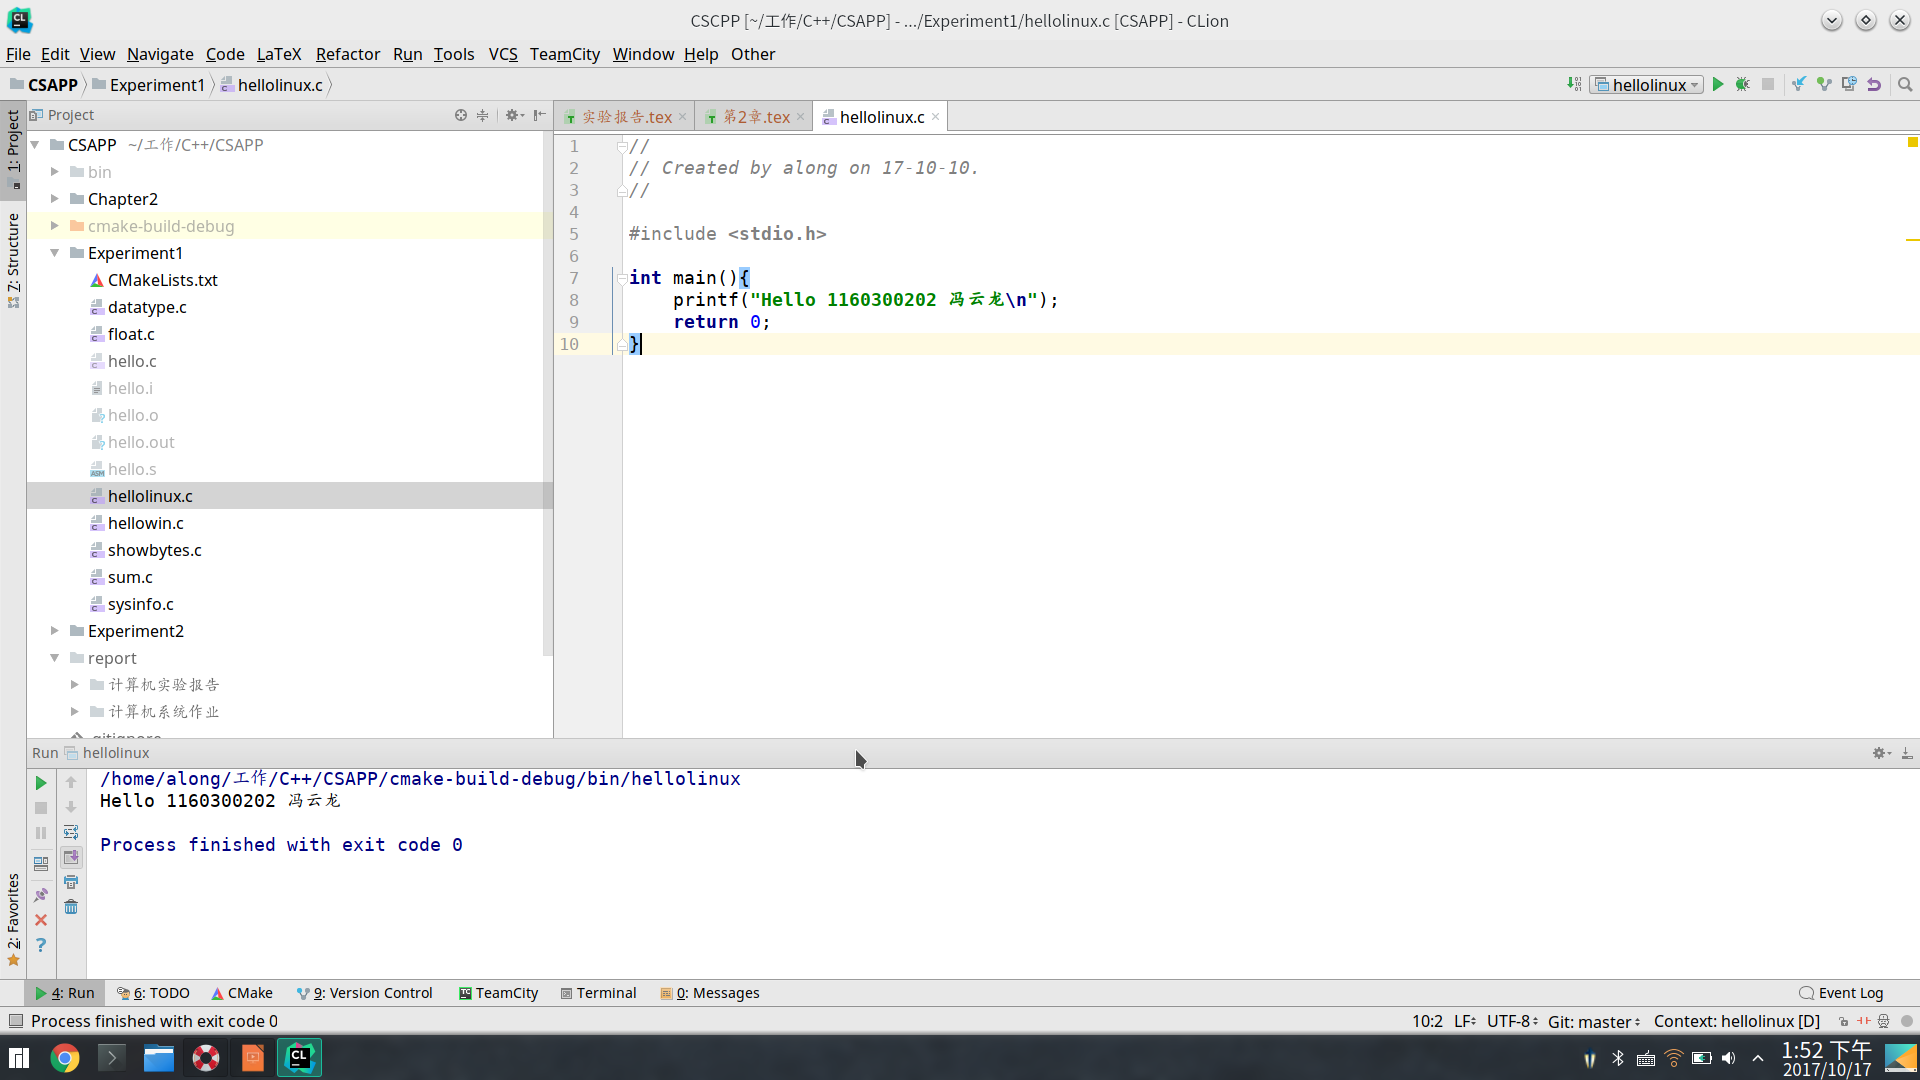
\includegraphics[width=0.55\linewidth]{figures/Linux-Clion}
	\caption{Linux下CLion截图}
	\label{fig:linux-clion}
\end{figure}

\subsection{Linux下EDB运行环境建立(10分)}

用EDB调试hellolinux.c的执行文件,截图,要求同 \ref{fig:linux-clion}。

\begin{figure}[H]
	\centering
	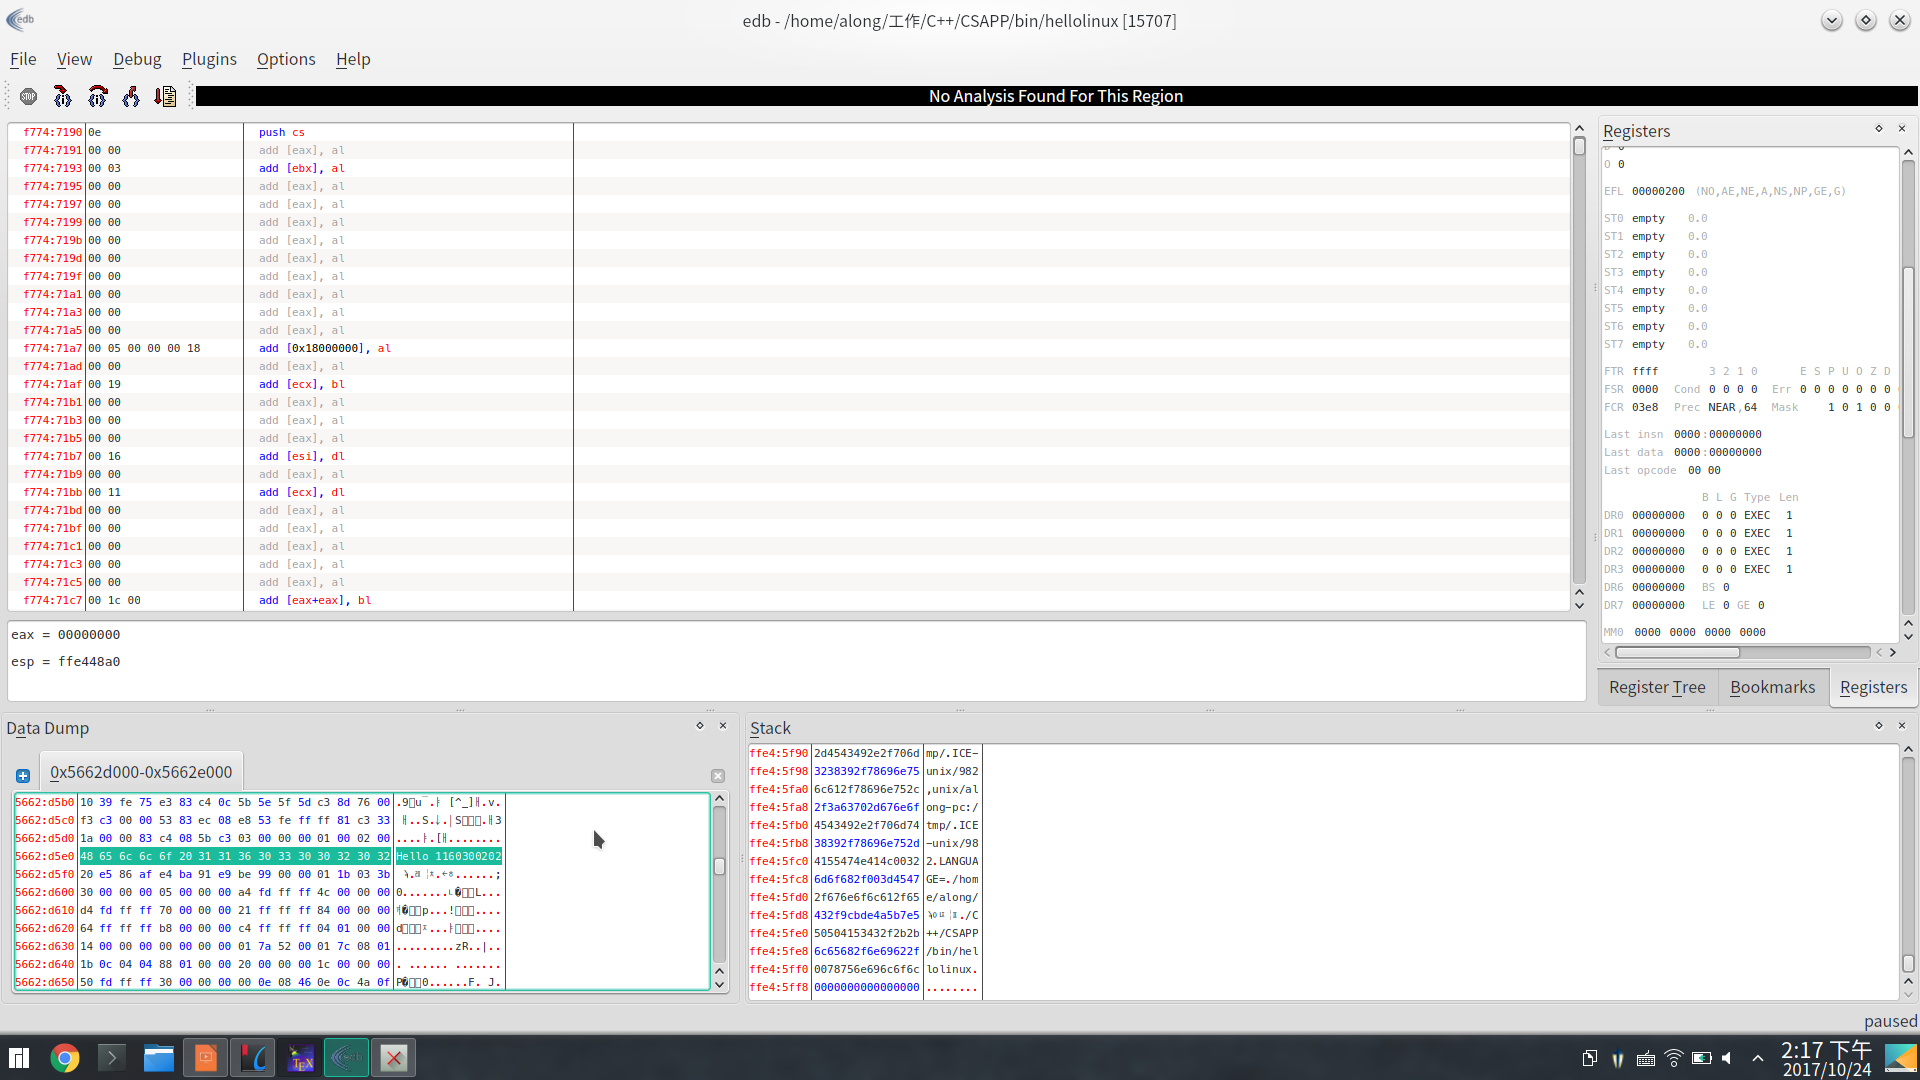
\includegraphics[width=0.5\linewidth]{figures/Linux-EDB}
	\caption{Linux下EDB截图}
	\label{linux-edb}
\end{figure}

